\documentclass[12pt]{report}

% Čeština
\usepackage[utf8]{inputenc}
\usepackage[IL2]{fontenc}
\usepackage[czech]{babel}

% Formát dokumentu
\usepackage{caption}
\usepackage{indentfirst}
\usepackage{graphicx}
\usepackage{textcomp}
\usepackage{amsmath}
\usepackage{parskip}
\usepackage{xspace}
\graphicspath{{img/}}
\usepackage[
left=30mm, 
right=30mm, 
top=30mm, 
bottom=30mm,
]{geometry}

% odstavec
\newcommand\myindent[1]{						
	\setlength\parindent{5mm}
	#1
	\setlength\parindent{0mm}
}											

\begin{document}
	
	% Titulní strana
	\begin{titlepage}
		\centering
		\Large
		
		
\includegraphics[width=.7\textwidth]{fav}
		
		\vspace{15mm}
		{\Huge\bfseries Identifikace spamu naivním bayesovským klasifikátorem}
		
		\vspace{15mm}
		{\LARGE Semestrální práce KIV/PC}
		
		\vfill
		\raggedright
		Mikuláš Mach\\
		A21B0202P
		\hfill 
		\today
	\end{titlepage}

	% Obsah
	\tableofcontents
	
	\chapter{Zadání}
	Naprogramujte v ANSI C přenositelnou \textbf{konzolovou aplikaci}, která bude \textbf{rozhodovat}, \textbf{zda úsek textu} (textový soubor předaný jako parametr na příkazové řádce) \textbf{je nebo není spam}.
	
	Program bude přijímat z příkazové řádky celkem \textbf{sedm} parametrů: První dva parametry budou
	vzor jména a počet trénovacích souborů obsahujících nevyžádané zprávy (tzv. \textbf{spam}). Třetí a
	čtvrtý parametr budou vzor jména a počet trénovacích souborů obsahujících vyžádané zprávy
	(tzv. \textbf{ham}). Pátý a šestý parametr budou vzor jména a počet testovacích souborů. Sedmý parametr představuje jméno výstupního textového souboru, který bude po dokončení činnosti Vašeho
	programu obsahovat výsledky klasifikace testovacích souborů.
	
	Program se tedy bude spouštět příkazem
		
	\myindent{spamid.exe ⟨spam⟩ ⟨spam-cnt⟩ ⟨ham⟩ ⟨ham-cnt⟩ ⟨test⟩ ⟨test-cnt⟩ ⟨out-file⟩}
	
	Symboly ⟨spam⟩, ⟨ham⟩ a ⟨test⟩ představují vzory jména vstupních souborů. Symboly ⟨spam-cnt⟩,
	⟨ham-cnt⟩ a ⟨test-cnt⟩ představují počty vstupních souborů. Vstupní soubory mají následující
	pojmenování: vzorN, kde N je celé číslo z intervalu ⟨1; N⟩. Přípona všech vstupních souborů je
	.txt, přípona není součástí vzoru. Váš program tedy může být během testování spuštěn například
	takto:
	
	\myindent{spamid.exe spam 10 ham 20 test 50 result.txt}
	
	Výsledkem činnosti programu bude textový soubor, který bude obsahovat seznam testovaných
	souborů a jejich klasifikaci (tedy rozhodnutí, zda je o spam či neškodný obsah~–~ham).


%-------------------------
%	Analýza úlohy
%-------------------------

	\chapter{Analýza úlohy}
	
	\section{Naivní bayesovský klasifikátor}
	
	Algoritmus má dvě fáze: \textbf{1) Fáze učení} a \textbf{2) Fáze klasifikace}.
	
		\subsection{Fáze učení}
		
		Načteme \textbf{slova} z \textbf{trénovacích souborů} a vytvoříme z nich \textbf{slovník}. Při načítání budeme vědět zda aktuálně načtené \textbf{slovo} patři do množiny \textbf{spam} nebo do množiny \textbf{ham}. Ve slovníku si budeme uchovávat u každého slova počet výskytů v každé množině. Následně vypočteme \textbf{podmíněnou pravděpodobnost výskytu slova} v \textbf{trénovacích souborech} pro množinu \textbf{spam} a pro množinu \textbf{ham} zvlášť. Využijeme tzv. \textit{bag-of-words}, to znamená že nám nebude záležet na pozici \textbf{slov}, ale jenom na jejich výskytu.
		
		\subsection{Fáze klasifikace}
		
		Zvlášť \textbf{počítáme pravděpodobnost} toho zda je \textbf{testovaný soubor} \textbf{spam} a zvlášť pravděpodobnost toho že je soubor \textbf{ham}. Ze souboru načteme \textbf{slovo}. Koukneme se jestli se \textbf{slovo} nachází ve \textbf{slovníku}, pokud ano, tak přičteme \textbf{logaritmus} jeho \textbf{podmíněné pravděpodobnosti výskytu} v dané množině k danému \textbf{výpočtu pravděpodobnosti}. Tento proces budeme opakovat dokud nenačteme všechny \textbf{slova} z \textbf{testovaného souboru}. Na konci dostaneme dvě čísla. Jedno udává jaká je \textbf{pravděpodobnost}, že \textbf{testovaný soubor} je \textbf{spam} a druhé udává pravděpodobnost toho že \textbf{soubor} je \textbf{ham}. Výpočet je popsán rovnicí \ref{Eq:vzorec} na straně \pageref{Eq:vzorec}.
		
		\clearpage
	
		\begin{equation}\label{Eq:vzorec}
			c = \arg\max_{c_i \in C} \left( \sum_{k\,\in\,\text{\bfseries pozice}} \log (P(⟨word_{k}⟩|c_{i})) \right)
		\end{equation}
	
	
	\begin{itemize}
		\item $C$ - Množina obsahující dvě podmnožiny (spam, ham)
		\item $c_i$ - Konkrétní prvek množiny
		\item $\arg\max$ - Pro všechny hodnoty $c_i$, vyčíslí hodnotu argumentu a vrátí $c_i$, pro kterou byla vypočtená hodnota nejvyšší
		\item $P(⟨word_{k}⟩|c_{i})$ – podmíněná pravděpodobnost výskytu slova
	\end{itemize}

%-------------------------
%	Datová struktura
%-------------------------

	\section{Datová struktura}
	
	Pro vytvoření \textbf{slovníku} bude nutné implementovat vhodnou \textbf{datovou strukturu}. \textbf{Struktura} by měla mít nízkou \textbf{časovou složitost} u vkládání a hledání prvku.
	
		\subsection{Spojový seznam}
		
		Na rozdíl od \textbf{pole} nebudeme muset u \textbf{spojového seznamu} řešit jeho velikost, protože se dá jednoduše rozšířit. \textbf{Spojový seznam} má \textbf{ukazatel} na jeho počáteční prvek tzv. \textit{head}, ten dále \textbf{ukazuje} právě na jeden další \textbf{prvek}. Všechny prvky jsou takhle \textbf{zřetězeny}. \textbf{Koncový prvek} má ukazatel nastavený na \textbf{NULL}. Spojový seznam je ukázán na obrázku \ref{fig:spojsez} na straně \pageref{fig:spojsez}. 
		
		\textbf{Operace vložení} má \textbf{časovou náročnost} O(1), pouze pokud si uložíme ukazatel i na \textbf{poslední prvek}, ale \textbf{operace nalezení prvku} má časovou složitost O(\textit{n}), tudíž je tato datová struktura \textbf{nevhodná} pro naší úlohu, protože \textbf{hledání prvku} bude často využíváno.
		
			\begin{figure}[h]
				\centering
				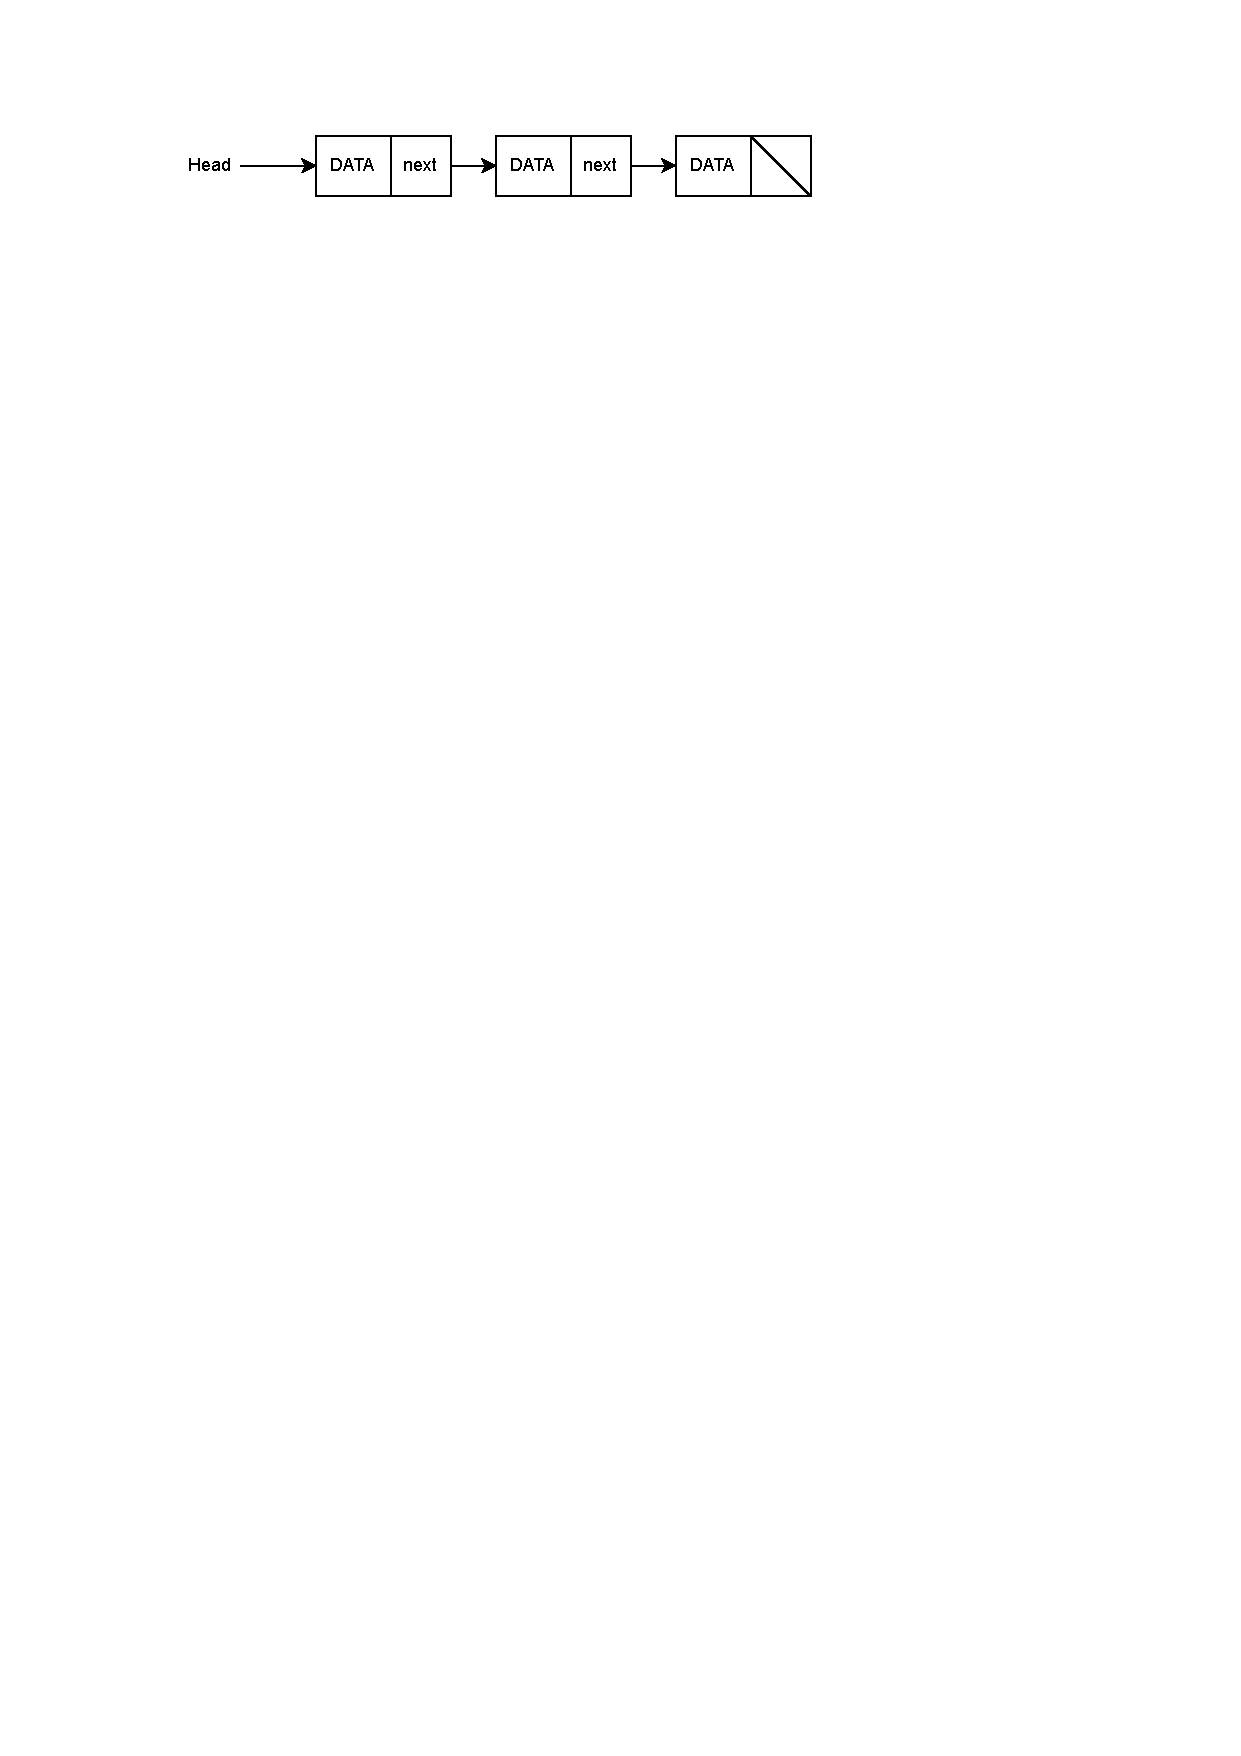
\includegraphics[width=.7\textwidth]{img/linkedlist}
				\caption{Spojový seznam}
				\label{fig:spojsez}
			\end{figure}
		
		\clearpage
		
		\subsection{Trie}
		
		\textbf{Trie} je \textit{"stromová"} struktura pro hledání specifického \textbf{klíče}. Někdy se taky nazývá jako \textbf{prefixový strom}. \textbf{Klíč} je do \textbf{trie} vložen po znacích jako posloupnost \textbf{uzlů}, tzn. že \textbf{vložení} má \textbf{časovou náročnost} O(\textit{k}), kde \textit{k} je \textbf{počet písmen} vkládaného klíče. Stejná časová složitost platí i pro \textbf{vyhledávání}. Na obrázku \ref{fig:trie} na straně \pageref{fig:trie} je ukázána \textbf{trie}, do které byla \textbf{vložena} slova: \textit{aha, ahoj, hell}.
		
		\begin{figure}[h]
			\centering
			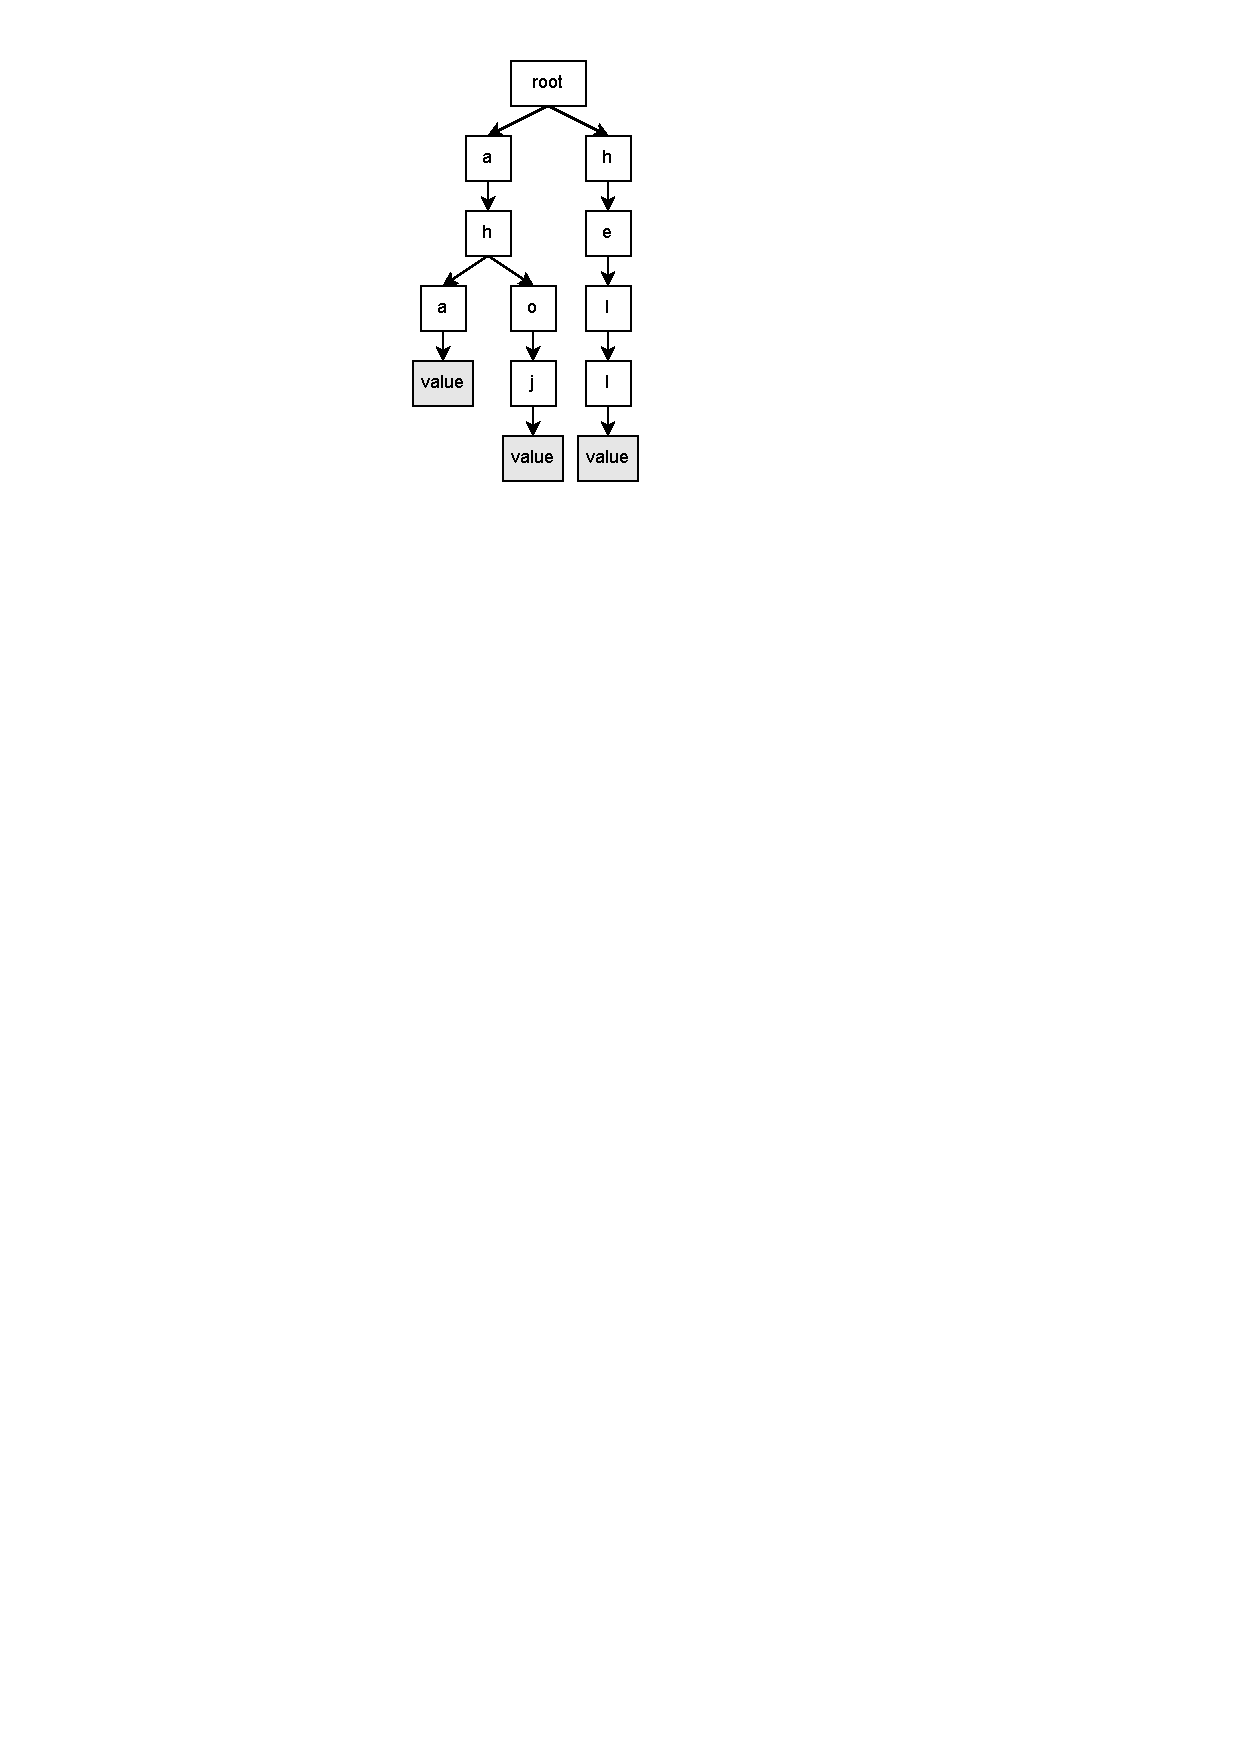
\includegraphics[width=.18\textwidth]{img/trie}
			\caption{Trie}
			\label{fig:trie}
		\end{figure}
		
		\subsection{Rozptýlená tabulka}
			
			Jedná se o \textbf{datovou strukturu}, která je postavena nad polem. Na rozdíl od normálního pole využívá \textit{hashovací funkci}. Díky této vlastnosti by \textbf{nalezení} i \textbf{vložení} daného \textbf{prvku} pomocí \textbf{klíče} mělo \textbf{průměrně} trvat O(1) a v \textbf{nejhorším případe} O(\textit{n}).
			
			V této datové struktuře může dojít ke \textbf{kolizi}, tzn. že při vložení různých \textbf{klíčů} do \textbf{hashovací funkce} dostaneme stejný výsledek. Tento problém by se řešil pomocí přidání \textbf{spojového seznamu} na každý index \textbf{tabulky}. Tím pádem nemůže dojít místo v \textbf{tabulce}. Pro zmenšení pravděpodobnosti \textbf{kolize} musí být \textbf{tabulka} dostatečně veliká a \textbf{hashovací funkce} musí dávat dostatečně \textbf{rozptýlené} hodnoty, ale zároveň nesmí být složitá, aby \textbf{nezpomalovala} program. Datová struktura je ukázána na obrázku \ref{fig:hashtable} na stráně \pageref{fig:hashtable}. 
			
			\begin{figure}[h]
				\centering
				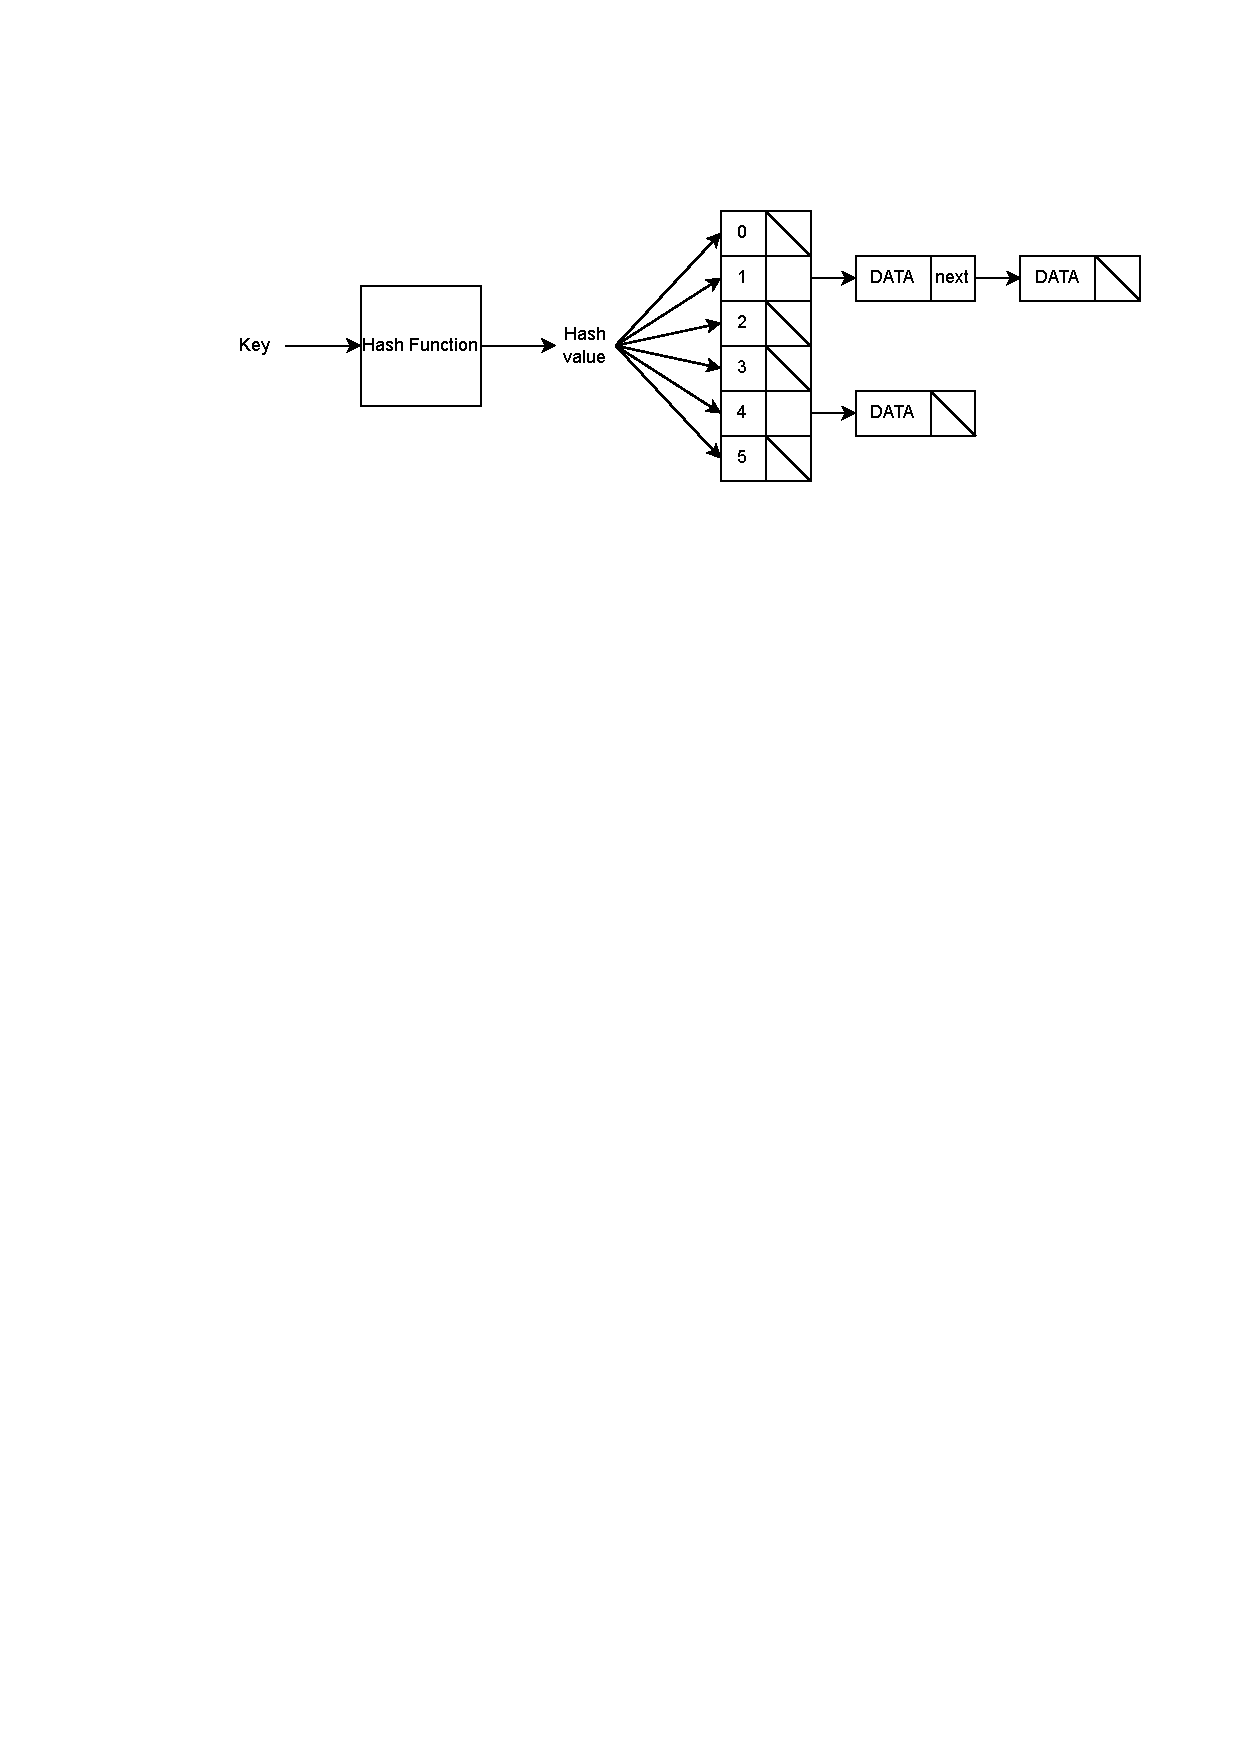
\includegraphics[width=.7\textwidth]{img/hashtable}
				\caption{Rozptýlená tabulka}
				\label{fig:hashtable}
			\end{figure}
		
		\subsection{Rozhodnutí}
		
		\textbf{Slovník} bude implementován pomocí \textbf{rozptýlené tabulky}, protože za použití dobré \textbf{hashovací funkce} dosáhneme dobré \textbf{časové náročnosti}, což v průměru je O(1) pro \textbf{vkládání} i pro \textbf{vyhledávání}.
		
		
%-------------------------
%	Implementace
%-------------------------

	\chapter{Implementace}
	
	Program je \textbf{rozdělen} na několik částí, konkrétně na: \textbf{Hashtable}, \textbf{Input}, \textbf{Bayes}, \textbf{Config} a \textbf{Main}. V části \textbf{Config} jsou pouze definice a v části \textbf{Main} jsou volány všechny důležité \textbf{funkce}.
	
	
	\section{Hashtable}
	
	Tabulka je využita jako \textbf{slovník}. Jsou v ní \textbf{uloženy} všechny hodnoty důležité pro \textbf{klasifikaci}. Tabulka obsahuje dvě \textbf{struktury}: \textbf{hashtable} a \textbf{item}.
	
		\subsection{Struktura item}
		
			Jedná se o \textbf{strukturu}, ve které jsou uložena data pro jedno konkrétní \textbf{slovo}. Tato \textbf{struktura} má představovat jednu položku v \textbf{tabulce}.
			Položka obsahuje svůj \textbf{klíč}, který je implementovaný jako řetězec charakterů, dále \textbf{obsahuje} obsahuje počet výskytů ve všech \textbf{spam souborech} a \textbf{podmíněnou pravděpodobnost výskytu}. \textbf{Struktura} má v sobě uloženy stejné \textbf{hodnoty} i pro všechny \textbf{ham soubory}. Poslední \textbf{uložená} věc ve \textbf{struktuře} je ukazatel na další \textbf{položku}, aby bylo možné \textbf{položky} zřetězit při \textbf{kolizi}.
				
		\subsection{Struktura hashtable}
		
			Jednoduchá \textbf{struktura}, která obsahuje \textbf{velikost tabulky}, počet vložení \textbf{slov typu spam}, počet vložení \textbf{slov typu ham} a pole \textbf{ukazatelů} typu \textbf{item}.
			
		\subsection{Funkce tabulky}
		
			\subsubsection{item\_create()}
		
			\textbf{Alokuje paměť} potřebnou pro \textbf{strukturu} a vloží do ní \textbf{klíč}. Jako \textbf{parametry} potřebuje \textbf{klíč} a číslo \textbf{0} (pokud \textbf{klíč} je ze \textbf{spam souboru}) nebo \textbf{1} (pokud klíč je z \textbf{ham souboru}).
			
			\subsubsection{hashtable\_create()}
		
			\textbf{Alokuje paměť} potřebnou pro \textbf{strukturu}, vloží do ní velikost tabulky a \textbf{alokuje} paměť pro \textbf{pole ukazatelů} typu \textbf{item}. 
			
			\subsubsection{hash()}
			
			Jako \textbf{parametry} přijímá \textbf{řetězech} a ukazatel na \textbf{tabulku} a vrací \textbf{index} v dané \textbf{tabulce}.
			
			\subsubsection{hashtable\_find()}
			
			Pomocí funkce \textbf{hash()} vypočte \textbf{index}, na kterém bude \textbf{vyhledávat}. Dokud nenarazí na \textbf{NULL}, tak bude \textbf{procházet} spojový seznam, který se nachází na daném \textbf{indexu}. Pokud funkce daný \textbf{item} nenajde, tak vrátí \textbf{NULL}, když ho najde, tak vrátí \textbf{ukazatel} na daný \textbf{item}.
			
			\subsubsection{add\_count()}
			
			Jako \textbf{parametry} přijímá \textbf{ukazatel na položku} a číslo \textbf{0} nebo \textbf{1}. Funkce pouze přičte jedničku buď k počtu výskytu dané položky ve \textbf{spam souborech} nebo \textbf{ham souborech} podle \textbf{číselného parametru}. Pokud byl parametr \textbf{0}, tak přičte k výskytu ve \textbf{spam souborech} a pokud \textbf{1}, tak k výskytu v \textbf{ham souborech}.
			
			\subsubsection{hashtable\_insert()}
			
			Funkce má jako parametry \textbf{ukazatel na tabulku}, \textbf{klíč} a číslo \textbf{0} (jedná se o \textbf{spam}) nebo \textbf{1} (jedná se o \textbf{ham}). Napřed pomocí funkce \textbf{hashtable\_find()} zjistí, jestli se prvek už nachází v tabulce, pokud ano, tak zavolá funkci \textbf{add\_count()} a funkce končí, pokud položka \textbf{nebyla nalezena}, tak zavolá funkci \textbf{item\_create()}. Následně pomocí funkce \textbf{hash()} vyhledá \textbf{index}, na který má \textbf{položku} vložit a projde spojový seznam, dokud nenarazí na \textit{"volné místo"}, kam následně \textbf{vytvořenou položku} vloží. Funkce vrátí číslo \textbf{1}, pokud vše proběhlo správně.
			
			
		\section{Input}
		
		Tato část programu se stará o \textbf{načítání trénovacích dat}.
		
		\subsection{Funkce}
		
			\subsubsection{read\_word()}
			
			Jako parametr přijímá \textbf{ukazatel} na \textbf{otevřený soubor}. 
			
			Funkce si \textbf{alokuje paměť} pro řetězec o předen \textbf{definované} velikosti. Následně funkce bude postupně číst znaky ze souboru a bude je vkládat do \textbf{řetězce}. Skončí až když narazí na \textbf{znak mezery} nebo na \textbf{konec souboru}. Po dokončení čtení se \textbf{alokuje} nový \textbf{řetězec}, který má stejnou velikost jako \textbf{počet načtených znaků} + 1 (\textbf{pro koncový znak}). Původní řetězec se \textbf{uvolní} a nově vytvořený \textbf{řetězec} funkce \textbf{vrátí jako výsledek}.
			
			\subsubsection{load()}
			
			Parametry funkce jsou: \textbf{ukazatel na tabulku}, \textbf{vzor názvu načínaných souborů} a \textbf{počet souborů}.
			
			Funkce si \textbf{alokuje paměť} pro řetězec. Ve \textbf{smyčce}  postupně \textbf{vytváří názvy trénovacích souborů}, pomocí \textbf{vzoru} a \textbf{počtu}.
			V této \textbf{smyčce} se nachází další \textbf{smyčka}, ve které se volá funkce \textbf{read\_word()}, dokud se nenarazí na konec souboru. Po načtení slova je \textbf{slovo vloženo} do \textbf{tabulky} pomocí \textbf{hashtable\_insert()}.
			
			
		\section{Bayes}
		
		V této části se provádí \textbf{klasifikace} testovaných souborů a všechny potřebné \textbf{výpočty}.
		
		\subsection{Funkce}
			
			\subsubsection{count()}
			Jednoduchá funkce, která přijme jako parametr \textbf{ukazatel na tabulku}. Projde přes všechny \textbf{prvky} v tabulce a \textbf{aktualizuje} počet vložených \textbf{slov typu ham} a počet vložených \textbf{slov typu spam}.
			
			\subsubsection{probabilities()}
			Jednoduchá funkce, která přijme jako parametr \textbf{ukazatel na tabulku}. Projde přes všechny \textbf{prvky} v tabulce a u každého z nich \textbf{vypočte} jejich \textbf{podmíněnou pravděpodobnost výskytu} v množině \textbf{spam} a v množině \textbf{ham}.
			
			\subsubsection{bayes\_one\_file()}
			Jako parametry přijímá: \textbf{Ukazatel na tabulku}, \textbf{řetězec s názvem testovaného souboru}, \textbf{ukazatel na otevřený výstupní soubor}.
			
			Tato funkce \textbf{klasifikuje} vždy jeden soubor. Uchovává si vždy \textbf{pravděpodobnost} toho, že soubor je \textbf{spam} a \textbf{pravděpodobnost} toho, že je \textbf{ham}. Funkce \textbf{otevře testovaný soubor} a bude ve smyčce pomocí funkce \textbf{read\_word()} číst soubor slovo po slově. Když načte slovo, tak se koukne do tabulky, když se tam nachází, tak přičte \textbf{zlogaritmovanou} danou \textbf{podmíněnou pravděpodobnost výskytu} k dané \textbf{uchovávané hodnotě}. Po průchodu celého souboru se \textbf{porovnají uchovávané hodnoty} a \textbf{klasifikujeme} soubor podle toho, která z nich je \textbf{větší}. \textbf{Výsledek} se \textbf{zapíše} do otevřeného \textbf{výstupního souboru}.
			
			\subsubsection{bayes()}
			
			Parametry funkce jsou: \textbf{Ukazatel na tabulku}, \textbf{řetězec vzoru názvu testovaných souborů}, \textbf{počet testovaných souborů}, \textbf{řetězec názvu výstupního souboru}.
			
			
			Funkce \textbf{alokuje paměť} pro řetězec a poté jsou zavolány funkce \textbf{count()} a \textbf{probabilities()}, aby bylo vše připraveno pro \textbf{klasifikaci}. Následuje smyčka, ve které jsou \textit{"skládány"} řetězce názvů \textbf{testovaných souborů}. Po každém \textit{"poskládání"} se zavolá funkce \textbf{bayes\_one\_file()}. Takto jsou postupně \textbf{klasifikovány} všechny souboru určené pro \textbf{testování}.
			
%-------------------------
%	Uživatelská příručka
%-------------------------			
			
	\chapter{Uživatelská příručka }
		
		\section{Přeložení programu}
		
			Pro překlad je využit \textbf{makefile}. Pro jeho funkci je nutné mít kompilátor \textbf{gcc} nebo \textbf{mingw}. Spouští se přes \textbf{terminál/příkazovou řádku}.
			Pro jeho spuštění musíme být ve stejném adresáři a použít příkaz \textbf{makefile} (pro gcc kompilátor) nebo příkaz \textbf{mingw32-make} (pro mingw kompilátor).
			
		\section{Spuštění programu}
		
			Po přeložení můžeme program spustit tímto příkazem:
			
			\myindent{spamid.exe ⟨spam⟩ ⟨spam-cnt⟩ ⟨ham⟩ ⟨ham-cnt⟩ ⟨test⟩ ⟨test-cnt⟩ ⟨out-file⟩}
			
			\begin{itemize}
				\item ⟨spam⟩, ⟨ham⟩ - Vzor názvu trénovacích spam a ham souborů
				\item ⟨spam-cnt⟩, ⟨ham-cnt⟩ - Počet trénovacích souborů
				\item ⟨test⟩ - Vzor názvu testovaných souborů
				\item ⟨test-cnt⟩ – Počet testovaných souborů
				\item ⟨out-file⟩ - Celý název výstupního souboru
			\end{itemize}
		
			Soubory pro trénování a testování se musí nacházet v \textbf{adresáři data}. Tento adresář musí být na stejné úrovni jako spouštěný program \textbf{spamid.exe}
			
			\textbf{Výstupní soubor} se vytvoří na stejné úrovni jako \textbf{spamid.exe}. Ve výstupním souboru je na každé řádce napsán název testovaného souboru a vedle toho je napsáno jak byl soubor \textbf{klasifikován}.
			
			Příklad příkazu pro spuštění:
			
			\myindent{spamid.exe spam 100 ham 100 test 10 result.txt}
			
%-------------------------
%	Závěr
%-------------------------
			
	\chapter{Závěr}
	
	Vytvořený program \textbf{splňuje} všechny body zadání. Klasifikace proběhne dostatečně rychle, přesnost klasifikace je vyšší než 90\% a program uvolňuje všechnu alokovanou paměť. \textbf{Kompilátor} při kompilaci neoznamuje žádné chyby.
	
	Program by mohl být navržen více \textbf{abstraktněji}. Například \textbf{hashtable}, tak jak je navržen teď, tak by s ničím jiným než s tímto zadáním nefungoval. Dále by šlo určitě dosáhnout rychlejšího běhu programu.
	
	Při klasifikaci jsem narazil na problém se vzorcem, který byl poskytnut v zadání. Po odstranění násobení \textbf{prior pravděpodobností}, klasifikace proběhla s dostatečnou přesností.
	Kromě tohoto problému jsem během implementace na žádný jiný problém nenarazil a všechno proběhlo v pořádku.
	
\end{document}